%{{第四回}}{第四回}}

\chapter{薄命女偏逢薄命郎\\葫芦僧乱判葫芦案}\label{part0008_split_000.htmlux5cux23calibre_pb_0}

{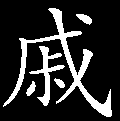
\includegraphics[width=3mm]{../Images/00005}\kaishu 阴阳交结变无伦,幻境生时即是真。秋月春花谁不见,朝晴暮雨自何因。心肝一点劳牵恋,可意偏长遇喜嗔。我爱世缘随分定,至诚相感作痴人。}

{\kaishu 请君着眼护官符,把笔悲伤说世途。作者泪痕同我泪,燕山仍旧窦公无。}

题曰:

捐躯报君恩,未报躯犹在。眼底物多情,君恩或可待。\href{../Text/part0008_split_000.html\#lnkback_1_a}{\textsuperscript{①}}

却说黛玉同姊妹们至王夫人处,见王夫人与兄嫂处的来使计议家务,又说姨母家遭人命官司等语。{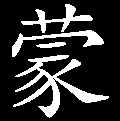
\includegraphics[width=3mm]{../Images/00006}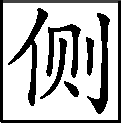
\includegraphics[width=3mm]{../Images/00011}\footnotesize \kaishu 又来一位,宝钗将出现矣。}因见王夫人事情冗杂,姊妹们遂出来,至寡嫂李氏房中来了。{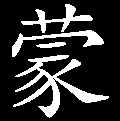
\includegraphics[width=3mm]{../Images/00006}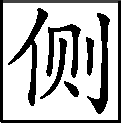
\includegraphics[width=3mm]{../Images/00011}\footnotesize \kaishu 慢慢度入法。}

原来这李氏即贾珠之妻。{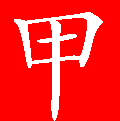
\includegraphics[width=3mm]{../Images/00002}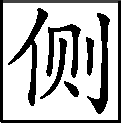
\includegraphics[width=3mm]{../Images/00011}\footnotesize \kaishu 起笔写薛家事,他偏写宫裁,是结黛玉,明李纨本末,又在人意料之外。}珠虽夭亡,幸存一子,取名贾兰,今已五岁,已入学攻书。这李氏亦系金陵名宦之女,父名李守中,{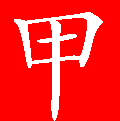
\includegraphics[width=3mm]{../Images/00002}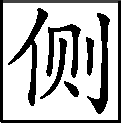
\includegraphics[width=3mm]{../Images/00011}\footnotesize \kaishu 妙!盖云人能以理自守,安得为情所陷哉!}曾为国子监祭酒,族中男女无有不诵诗读书者。{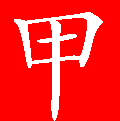
\includegraphics[width=3mm]{../Images/00002}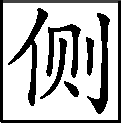
\includegraphics[width=3mm]{../Images/00011}\footnotesize \kaishu 未出李纨,先伏下李纹、李绮。}至李守中承继以来,便说``女儿无才便有{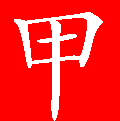
\includegraphics[width=3mm]{../Images/00002}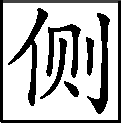
\includegraphics[width=3mm]{../Images/00011}\footnotesize \kaishu ``有''字改得好。}德'',{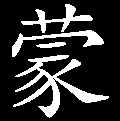
\includegraphics[width=3mm]{../Images/00006}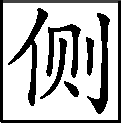
\includegraphics[width=3mm]{../Images/00011}\footnotesize \kaishu 确论。}故生了李氏时,便不十分令其读书,只不过将些《女四书》、《列女传》、《贤媛集》等三四种书,使他认得几个字、记得这前朝几个贤女便罢了,却只以纺绩井臼为要,因取名为李纨,字宫裁。{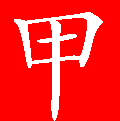
\includegraphics[width=3mm]{../Images/00002}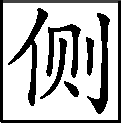
\includegraphics[width=3mm]{../Images/00011}\footnotesize \kaishu 一洗小说窠臼俱尽,且命名字,亦不见红香翠玉恶俗。}因此这李纨虽青春丧偶,且居处于膏粱锦绣之中,竟如槁木死灰一般,{{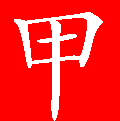
\includegraphics[width=3mm]{../Images/00002}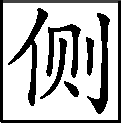
\includegraphics[width=3mm]{../Images/00011}\footnotesize \kaishu 此时处此境,最能越{(理)}{[}礼{]}生事,彼竟不然,实罕见者。 }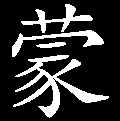
\includegraphics[width=3mm]{../Images/00006}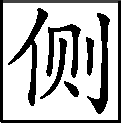
\includegraphics[width=3mm]{../Images/00011}\footnotesize \kaishu 反有此等文章。}一概无见无闻,唯知侍亲养子,外则陪侍小姑等针黹诵读而已。{{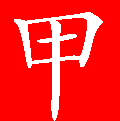
\includegraphics[width=3mm]{../Images/00002}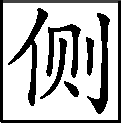
\includegraphics[width=3mm]{../Images/00011}\footnotesize \kaishu 一段叙出李纨,不犯熙凤。 }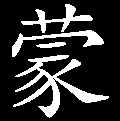
\includegraphics[width=3mm]{../Images/00006}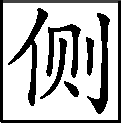
\includegraphics[width=3mm]{../Images/00011}\footnotesize \kaishu 此中不得不有如此人。天地覆载,何物不有?而才子手中,亦何物不有?}今黛玉虽客寄于斯,日有这般姐妹相伴,除老父外,馀者也就无庸虑及了。{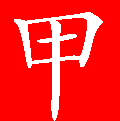
\includegraphics[width=3mm]{../Images/00002}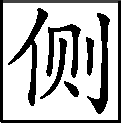
\includegraphics[width=3mm]{../Images/00011}\footnotesize \kaishu 仍是从黛玉身上写来,以上了结住黛玉,复找前文。}

如今且说贾雨村,因补授了应天府,一下马,就有一件人命官司详至案下,{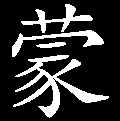
\includegraphics[width=3mm]{../Images/00006}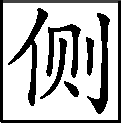
\includegraphics[width=3mm]{../Images/00011}\footnotesize \kaishu 非雨村难以了结此案。}乃是两家争买一婢,各不相让,以致殴伤人命。彼时雨村即问原告。那原告道:``被殴死者乃小人之主人。因那日买了一个丫头,不想系拐子所拐来卖的。这拐子先已得了我家银子,我家小爷原说第三日方是好日子,再接入门。{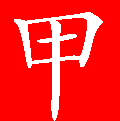
\includegraphics[width=3mm]{../Images/00002}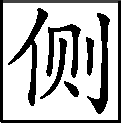
\includegraphics[width=3mm]{../Images/00011}\footnotesize \kaishu 所谓``迟则有变'',往往世人因不经之谈误却大事。}这拐子便又悄悄的卖与了薛家,被我们知道了,去找那卖主夺取丫头。无奈薛家原系金陵一霸,倚财仗势,众豪奴将我主人竟打死了。{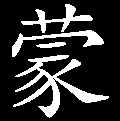
\includegraphics[width=3mm]{../Images/00006}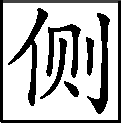
\includegraphics[width=3mm]{../Images/00011}\footnotesize \kaishu 一派世境恶习活现。}凶身主仆已皆逃走,无影无踪,只剩了几个局外之人。小人告了一年的状,竟无人作主。{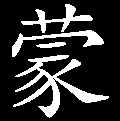
\includegraphics[width=3mm]{../Images/00006}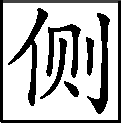
\includegraphics[width=3mm]{../Images/00011}\footnotesize \kaishu 悲夫!千古世情,不过如此。}望大老爷拘拿凶犯,剪恶除凶,以救孤寡,死者感戴天恩不尽!''

雨村听了大怒{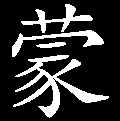
\includegraphics[width=3mm]{../Images/00006}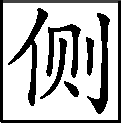
\includegraphics[width=3mm]{../Images/00011}\footnotesize \kaishu 偏能用反跌法。}道:``岂有这样放屁的事!打死人命就白白的走了,再拿不来的?''因发签差公人立刻将凶犯族中人拿来拷问,令他们实供藏在何处,一面再动海捕文书。正要发签时,只见案边立着一个门子,使眼色儿不令他发签之意。雨村心中甚是疑怪,{{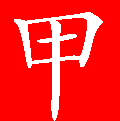
\includegraphics[width=3mm]{../Images/00002}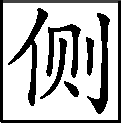
\includegraphics[width=3mm]{../Images/00011}\footnotesize \kaishu 原可疑怪,余亦疑怪。 }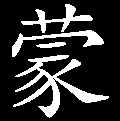
\includegraphics[width=3mm]{../Images/00006}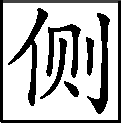
\includegraphics[width=3mm]{../Images/00011}\footnotesize \kaishu 请看文字递出递转,闲中皆是要笔。}只得停了手。即时退堂,至密室,使从皆退去,只留下门子一人伏侍。这门子忙上来请安,笑问:``老爷一向加官进禄,八九年来就忘了我了?''{{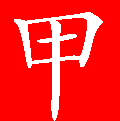
\includegraphics[width=3mm]{../Images/00002}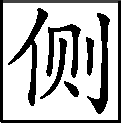
\includegraphics[width=3mm]{../Images/00011}\footnotesize \kaishu 语气傲慢,怪甚! }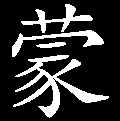
\includegraphics[width=3mm]{../Images/00006}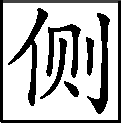
\includegraphics[width=3mm]{../Images/00011}\footnotesize \kaishu 似闲语,是要人。}雨村道:``却十分面善得紧,只是一时想不起来。''那门子笑道:``老爷真是贵人多忘事,把出身之地竟忘了,{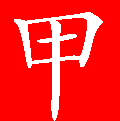
\includegraphics[width=3mm]{../Images/00002}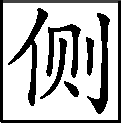
\includegraphics[width=3mm]{../Images/00011}\footnotesize \kaishu 刹心语。自招其祸,亦因夸能恃才也。}不记当年葫芦庙里之事了?''雨村听了,如雷震一惊,{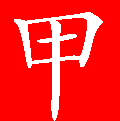
\includegraphics[width=3mm]{../Images/00002}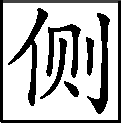
\includegraphics[width=3mm]{../Images/00011}\footnotesize \kaishu 余亦一惊,但不知门子何知,尤为怪甚。}方想起往事。原来这门子本是葫芦庙内一个小沙弥,因被火之后,无处安身,欲投别庙去修行,又耐不得清凉景况,因想这件生意倒还轻省热闹,{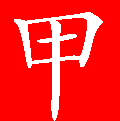
\includegraphics[width=3mm]{../Images/00002}\includegraphics[width=3mm]{../Images/00011}\footnotesize \kaishu 新鲜字眼。}遂趁年纪蓄了发,充了门子。{\includegraphics[width=3mm]{../Images/00002}\includegraphics[width=3mm]{../Images/00011}\footnotesize \kaishu 一路奇奇怪怪,调侃世人,总在人意臆之外。}雨村那里料得是他,便忙携手笑道:``原来是故人。''{\includegraphics[width=3mm]{../Images/00002}\includegraphics[width=3mm]{../Images/00011}\footnotesize \kaishu 妙称!全是假态。}又让坐了好谈。{\includegraphics[width=3mm]{../Images/00002}\includegraphics[width=3mm]{../Images/00011}\footnotesize \kaishu 假极!}这门子不敢坐。雨村笑道:``贫贱之交不可忘,{\includegraphics[width=3mm]{../Images/00002}\includegraphics[width=3mm]{../Images/00011}\footnotesize \kaishu 全是奸险小人态度,活现活跳。}你我故人也,二则此系私室,{\includegraphics[width=3mm]{../Images/00006}\includegraphics[width=3mm]{../Images/00011}\footnotesize \kaishu 如此亲近,其先必有故事。}既欲长谈,岂有不坐之理?''这门子听说,方告了座,斜签着坐了。

雨村因问方才何故不令发签。这门子道:``老爷既荣任到这一省,难道就没抄一张`护官符'{\includegraphics[width=3mm]{../Images/00002}\includegraphics[width=3mm]{../Images/00011}\footnotesize \kaishu 可对``聚宝盆'',一笑。◇三字从来未见,奇之至!}来不成?''雨村忙问:``何为`护官符'?{\includegraphics[width=3mm]{../Images/00002}\includegraphics[width=3mm]{../Images/00011}\footnotesize \kaishu 余亦欲问。}我竟不知。''门子道:``这还了得!连这不知,怎能作得长远!{{\includegraphics[width=3mm]{../Images/00002}\includegraphics[width=3mm]{../Images/00011}\footnotesize \kaishu 骂得爽快! }\includegraphics[width=3mm]{../Images/00006}\includegraphics[width=3mm]{../Images/00011}\footnotesize \kaishu 真是警世之言。使我看之,不知要哭要笑。}如今凡作地方官者,皆有一个私单,上面写的是本省最有权有势、极富极贵的大乡绅名姓,各省皆然。倘若不知,一时触犯了这样的人家,不但官爵,只怕连性命还保不成呢!{{\includegraphics[width=3mm]{../Images/00002}\includegraphics[width=3mm]{../Images/00011}\footnotesize \kaishu 可怜可叹,可恨可气,变作一把眼泪也。 }\includegraphics[width=3mm]{../Images/00006}\includegraphics[width=3mm]{../Images/00011}\footnotesize \kaishu 快论。请问其言是乎否乎?}所以绰号叫作`护官符'。{\includegraphics[width=3mm]{../Images/00002}\includegraphics[width=3mm]{../Images/00011}\footnotesize \kaishu 奇甚趣甚,如何想来?}方才所说的这薛家,老爷如何惹得他!他这一件官司并无难断之处,皆因都碍着情分脸面,所以如此。''一面说,一面从顺袋中取出一张抄写的`护官符'来,递与雨村,看时,上面皆是本地大族名宦之家的谚俗口碑。其口碑排写得明白,下面皆注着始祖官爵并房次。{\includegraphics[width=3mm]{../Images/00005}\includegraphics[width=3mm]{../Images/00012}\footnotesize \kaishu 此等人家,岂必欺霸方始成名耶?总因子弟不肖,招接匪人,一朝生事则百计营求,父为子隐,群小迎合,虽暂时不罹祸网,而从此放胆,必破家灭族不已,哀哉! \includegraphics[width=3mm]{../Images/00006}\includegraphics[width=3mm]{../Images/00011}\footnotesize \kaishu 可怜伊等始祖。}石头亦曾照样抄写一张,{\includegraphics[width=3mm]{../Images/00002}\includegraphics[width=3mm]{../Images/00011}\footnotesize \kaishu 忙中闲笔,用得好。}今据石上所抄云:

贾不假,白玉为堂金作马。{\includegraphics[width=3mm]{../Images/00002}\includegraphics[width=3mm]{../Images/00011}\footnotesize \kaishu 宁国、荣国二公之后,共二十房分,除宁、荣亲派八房在都外,现原籍住者十二房。}

阿房宫,三百里,住不下金陵一个史。{\includegraphics[width=3mm]{../Images/00002}\includegraphics[width=3mm]{../Images/00011}\footnotesize \kaishu 保龄侯尚书令史公之后,房分共十八。都中现住者十房,原籍现居八房。}

丰年好大雪,{\includegraphics[width=3mm]{../Images/00002}\includegraphics[width=3mm]{../Images/00012}\footnotesize \kaishu 隐``薛''字。}珍珠如土金如铁。{\includegraphics[width=3mm]{../Images/00002}\includegraphics[width=3mm]{../Images/00011}\footnotesize \kaishu 紫微舍人薛公之后,现领内府帑银行商,共八房分。}

东海缺少白玉床,龙王来请金陵王。{\includegraphics[width=3mm]{../Images/00002}\includegraphics[width=3mm]{../Images/00011}\footnotesize \kaishu 都太尉统制县伯王公之后,共十二房。都中二房,馀皆在籍。}\href{../Text/part0008_split_000.html\#lnkback_2_a}{\textsuperscript{②}}

雨村犹未看完,{\includegraphics[width=3mm]{../Images/00002}\includegraphics[width=3mm]{../Images/00010}\footnotesize \kaishu 妙极!若只有此四家,则死板不活,若再有两家,又觉累赘,故如此断法。}忽闻传点人报:``王老爷来拜。''雨村听说,忙具衣冠出去迎接。{\includegraphics[width=3mm]{../Images/00002}\includegraphics[width=3mm]{../Images/00011}\footnotesize \kaishu 横云断岭法,是板定大章法。}有顿饭工夫,方回来细问。这门子道:``这四家皆连络有亲,一损皆损,一荣皆荣,扶持遮饰,皆有照应的。{{\includegraphics[width=3mm]{../Images/00002}\includegraphics[width=3mm]{../Images/00011}\footnotesize \kaishu 早为下半部伏根。 }\includegraphics[width=3mm]{../Images/00006}\includegraphics[width=3mm]{../Images/00011}\footnotesize \kaishu 此四家不相为结亲,则无门当户对者,亦理势之必然。既结亲之后,岂不照应,又人情之不可无。}今告打死人之薛,就系`丰年大雪'之薛也。不单靠这三家,他的世交亲友在都在外者,本亦不少。老爷如今拿谁去?''雨村听如此说,便笑问门子道:``如你这样说来,却怎么了结此案?你大约也深知这凶犯躲的方向了?''

门子笑道:``不瞒老爷说,不但这凶犯躲的方向我知道,一并这拐卖之人{\includegraphics[width=3mm]{../Images/00002}\includegraphics[width=3mm]{../Images/00011}\footnotesize \kaishu 斯何人也。}我也知道,死鬼买主也深知道。待我细说与老爷听:{\includegraphics[width=3mm]{../Images/00006}\includegraphics[width=3mm]{../Images/00011}\footnotesize \kaishu 放胆一说,毫无避忌。世态人情被门子参透了。}这个被打之死鬼,乃是本地一个小乡宦之子,名唤冯渊,{\includegraphics[width=3mm]{../Images/00002}\includegraphics[width=3mm]{../Images/00011}\footnotesize \kaishu 真真是冤孽相逢。}自幼父母早亡,又无兄弟,只他一个人守着些薄产过日。{\includegraphics[width=3mm]{../Images/00006}\includegraphics[width=3mm]{../Images/00011}\footnotesize \kaishu 我为幼而失父母者一哭。}长到十八九岁上,酷爱男风,最厌女子。{\includegraphics[width=3mm]{../Images/00002}\includegraphics[width=3mm]{../Images/00011}\footnotesize \kaishu 最厌女子,仍为女子丧生,是何等大笔!不是写冯渊,正是写英莲。}这也是前生冤孽,可巧{\includegraphics[width=3mm]{../Images/00002}\includegraphics[width=3mm]{../Images/00011}\footnotesize \kaishu 善善恶恶,多从可巧而来,可畏可怕。}遇见这拐子卖丫头,他便一眼看上了这丫头,立意买来作妾,立誓再不交结男子,{\includegraphics[width=3mm]{../Images/00002}\includegraphics[width=3mm]{../Images/00011}\footnotesize \kaishu 谚云:``人若改常,非病即亡。''信有之乎?}也再不娶第二个了,{{\includegraphics[width=3mm]{../Images/00002}\includegraphics[width=3mm]{../Images/00011}\footnotesize \kaishu 虚写一个情种。 }\includegraphics[width=3mm]{../Images/00006}\includegraphics[width=3mm]{../Images/00011}\footnotesize \kaishu 也是幻中情魔。}所以三日后方过门。谁晓这拐子又偷卖与了薛家,{\includegraphics[width=3mm]{../Images/00006}\includegraphics[width=3mm]{../Images/00011}\footnotesize \kaishu 一定情即了结,请问是幻不是?点醒幻字,人皆不醒。我今日看了、批了,仍也是不醒。}他意欲卷了两家银子,再逃往他省。谁知又不曾走脱,两家拿住,打了个臭死,都不肯收银,只要领人。那薛家公子岂是让人的,便喝着手下人一打,将冯公子打了个稀烂,{\includegraphics[width=3mm]{../Images/00006}\includegraphics[width=3mm]{../Images/00011}\footnotesize \kaishu 有情反是无情。}抬回家去,三日死了。这薛公子原是早已择定日子上京去的,头起身两日前,就偶然遇见了这丫头,意欲买了就进京的,谁知闹出这事来。既打了冯公子,夺了丫头,他便没事人一般,只管带了家眷走他的路。他这里自有兄弟奴仆在此料理,并不为此些些小事值得他一逃走的。{\includegraphics[width=3mm]{../Images/00002}\includegraphics[width=3mm]{../Images/00011}\footnotesize \kaishu 妙极!人命视为``些些小事'',总是刻画阿呆耳。}这且别说,老爷你当被卖之丫头是谁?''{\includegraphics[width=3mm]{../Images/00002}\includegraphics[width=3mm]{../Images/00011}\footnotesize \kaishu 问得又怪。}雨村道:``我如何得知?''门子冷笑道:``这人算来还是老爷的大恩人呢!{\includegraphics[width=3mm]{../Images/00006}\includegraphics[width=3mm]{../Images/00011}\footnotesize \kaishu 当心一脚。请看后文,并无蹴动。}他就是葫芦庙旁住的甄老爷的小姐,名唤英莲的。''{\includegraphics[width=3mm]{../Images/00002}\includegraphics[width=3mm]{../Images/00011}\footnotesize \kaishu 至此一醒。}雨村罕然道:``原来就是他!闻得养至五岁被人拐去,却如今才来卖呢?''{\includegraphics[width=3mm]{../Images/00006}\includegraphics[width=3mm]{../Images/00011}\footnotesize \kaishu ``闻得''只说一层,并无言及要娇杏自道{(子)}{[}之{]}语。非作者忘怀,欲写世态,故作幻笔。}

门子道:``这一种拐子单管偷拐五六岁的儿女,养在一个僻静之处,到十一二岁时,度其容貌,带至他乡转卖。当日这英莲我们天天哄他顽耍,虽隔了七八年,如今十二三岁的光景,其模样虽然出脱得齐整好些,然大概相貌,自是不改,熟人易认。况且他眉心中原有米粒大小的一点胭脂?,从胎里带来的,{{{\includegraphics[width=3mm]{../Images/00002}\includegraphics[width=3mm]{../Images/00011}\footnotesize \kaishu 宝钗之热,黛玉之怯,悉从胎中带来。今英莲有}?{,其人可知矣。}}}所以我却认得。偏生这拐子又租了我的房舍居住,{\includegraphics[width=3mm]{../Images/00005}\includegraphics[width=3mm]{../Images/00012}\footnotesize \kaishu 作者要说容貌势力,要说情,要说幻,又要说小人之居心,豪强之托大,了结前文旧案,铺设后文根基。点明英莲,收叙宝钗等项诸事:只借先之沙弥、今日门子之口层层叙来,真是大悲菩萨,千手千眼一时转动,毫无遗露。可见具大光明者,故无难事,诚然。}那日拐子不在家,我也曾问他。他是被拐子打怕了的,{{\includegraphics[width=3mm]{../Images/00002}\includegraphics[width=3mm]{../Images/00011}\footnotesize \kaishu 可怜! }\includegraphics[width=3mm]{../Images/00006}\includegraphics[width=3mm]{../Images/00011}\footnotesize \kaishu 世家子女至此。可想见其先世亦必有如薛公子者。}万不敢说,只说拐子系他亲爹,因无钱偿债,故卖他。我又哄之再四,他又哭了,{\includegraphics[width=3mm]{../Images/00006}\includegraphics[width=3mm]{../Images/00011}\footnotesize \kaishu 写其心机,总为后文。}只说:`我原不记得小时之事!'这可无疑了。那日冯公子相看了,兑了银子,拐子醉了,他自叹道:`我今日罪孽可满了!'{\includegraphics[width=3mm]{../Images/00006}\includegraphics[width=3mm]{../Images/00011}\footnotesize \kaishu 天下英雄,失足匪人,偶得机会可以跳出者,与英莲同声一哭!}后又听得冯公子三日后才娶过门,他又转有忧愁之态。我又不忍其形景,等拐子出去,又命内人去解释他:`这冯公子必待好日期来接,可知必不以丫鬟相看。况他是个绝风流人品,家里颇过得,素习又最厌恶堂客,今竟破价买你,后事不言可知。只耐得三两日,何必忧闷!'{\includegraphics[width=3mm]{../Images/00006}\includegraphics[width=3mm]{../Images/00011}\footnotesize \kaishu 良人者所望而终身也。}他听如此说,方才略解忧闷,自为从此得所。谁料天下竟有这等不如意事,{{\includegraphics[width=3mm]{../Images/00002}\includegraphics[width=3mm]{../Images/00011}\footnotesize \kaishu 可怜真可怜!◇一篇《薄命赋》,特出英莲。 }\includegraphics[width=3mm]{../Images/00006}\includegraphics[width=3mm]{../Images/00011}\footnotesize \kaishu 天下同患难者同来一哭!}第二日,他偏又卖与了薛家。若卖与第二个人还好,这薛公子的混名人称`呆霸王',最是天下第一个弄性尚气的人,而且使钱如土,{{\includegraphics[width=3mm]{../Images/00002}\includegraphics[width=3mm]{../Images/00011}\footnotesize \kaishu 世路难行钱作马。 }\includegraphics[width=3mm]{../Images/00006}\includegraphics[width=3mm]{../Images/00011}\footnotesize \kaishu ``使钱如土'',方能称霸王。}遂打了个落花流水,生拖死拽,把个英莲拖去,如今也不知死活。{\includegraphics[width=3mm]{../Images/00002}\includegraphics[width=3mm]{../Images/00011}\footnotesize \kaishu 为英莲留后步。}这冯公子空喜一场,一念未遂,反花了钱,送了命,岂不可叹!''{\includegraphics[width=3mm]{../Images/00002}\includegraphics[width=3mm]{../Images/00010}\footnotesize \kaishu 又一首《薄命叹》。英、冯二人一段小悲欢幻景从葫芦僧口中补出,省却闲文之法也。所谓``美中不足,好事多魔'',先用冯渊作一开路之人。}

雨村听了,亦叹道:``这也是他们的孽障遭遇,亦非偶然。不然这冯渊如何偏只看准了这英莲?这英莲受了拐子这几年折磨,才得了个头路,且又是个多情的,若能聚合了,倒是一件美事,偏又生出这段事来。{\includegraphics[width=3mm]{../Images/00006}\includegraphics[width=3mm]{../Images/00011}\footnotesize \kaishu 冯渊之事之人,是英莲之幻景中之痴情人。}这薛家纵比冯家富贵,想其为人,自然姬妾众多,淫佚无度,未必及冯渊定情于一人者。这正是梦幻情缘,{\includegraphics[width=3mm]{../Images/00006}\includegraphics[width=3mm]{../Images/00011}\footnotesize \kaishu 点明白了,直入本题。}恰遇见一对薄命儿女。{\includegraphics[width=3mm]{../Images/00002}\includegraphics[width=3mm]{../Images/00010}\footnotesize \kaishu 使雨村一评,方补足上半回之题目。所谓此书有繁处愈繁,省中愈省;又有不怕繁中繁,只要繁中虚;不畏省中省,只要省中实。此则省中实也。}且不要议论他,只目今这官司,如何剖断才好?''门子笑道:``老爷当年何等明决,今日何翻成个没主意的人了!{\includegraphics[width=3mm]{../Images/00006}\includegraphics[width=3mm]{../Images/00011}\footnotesize \kaishu 利欲薰心,必致如此。}小的闻得老爷补升此任,亦系贾府、王府之力,此薛蟠即贾府之老亲,老爷何不顺水行舟,做个整人情,将此案了结,日后也好见贾、王二公的。''雨村道:``你说的何尝不是。{\includegraphics[width=3mm]{../Images/00002}\includegraphics[width=3mm]{../Images/00011}\footnotesize \kaishu 可发一长叹。这一句已见奸雄,全是假。}但事关人命,蒙皇上隆恩,起复委用,{\includegraphics[width=3mm]{../Images/00002}\includegraphics[width=3mm]{../Images/00011}\footnotesize \kaishu 奸雄。}实是重生再造,正当殚心竭力图报之时,{\includegraphics[width=3mm]{../Images/00002}\includegraphics[width=3mm]{../Images/00011}\footnotesize \kaishu 奸雄。}岂可因私而废法?{{\includegraphics[width=3mm]{../Images/00002}\includegraphics[width=3mm]{../Images/00011}\footnotesize \kaishu 奸雄。 }\includegraphics[width=3mm]{../Images/00006}\includegraphics[width=3mm]{../Images/00011}\footnotesize \kaishu 良明不昧势难当。}是我实不能忍为者。''{\includegraphics[width=3mm]{../Images/00002}\includegraphics[width=3mm]{../Images/00011}\footnotesize \kaishu 全是假。}门子听了,冷笑道:``老爷说的何尝不是大道理,但只是如今世上是行不去的。岂不闻古人有云`大丈夫相时而动',{\includegraphics[width=3mm]{../Images/00006}\includegraphics[width=3mm]{../Images/00011}\footnotesize \kaishu 误尽多少苍生!}又曰`趋吉避凶者为君子'。{\includegraphics[width=3mm]{../Images/00002}\includegraphics[width=3mm]{../Images/00011}\footnotesize \kaishu 近时错会书意者多多如此。}依老爷这一说,不但不能报效朝廷,亦且自身不保,{\includegraphics[width=3mm]{../Images/00006}\includegraphics[width=3mm]{../Images/00011}\footnotesize \kaishu 说了来也是一团道理。}还要三思为妥。''

雨村低了半日头,{\includegraphics[width=3mm]{../Images/00002}\includegraphics[width=3mm]{../Images/00011}\footnotesize \kaishu 奸雄欺人。}方说道:``依你怎么样?''门子道:``小人已想了个极好的主意在此:老爷明日坐堂,只管虚张声势,动文书发签拿人。原凶自然是拿不来的,原告固是定要将薛家族中及奴仆人等拿几个来拷问。小的在暗中调停,令他们报个暴病身亡,合族中及地方上共递一张保呈,老爷只说善能扶鸾请仙,堂上设下乩坛,令军民人等只管来看。老爷就说:`乩仙批了,死者冯渊与薛蟠原因夙孽相逢,今狭路既遇,原应了结。薛蟠今已得无名之症,{\includegraphics[width=3mm]{../Images/00002}\includegraphics[width=3mm]{../Images/00011}\footnotesize \kaishu ``无名之症''却是病之名,而反曰``无'',妙极!}被冯魂追索已死。其祸皆由拐子某人而起,拐之人原系某乡某姓人氏,按法处治,馀不略及'等语。小人暗中嘱托拐子,令其实招。众人见乩仙批语与拐子相符,馀者自然也都不虚了。薛家有的是钱,老爷断一千也可,五百也可,与冯家作烧埋之费。那冯家也无甚要紧的人,不过为的是钱,见有了这个银子,想也就无话了。老爷细想此计如何?''雨村笑道:``不妥,不妥。{\includegraphics[width=3mm]{../Images/00002}\includegraphics[width=3mm]{../Images/00011}\footnotesize \kaishu 奸雄欺人。}等我再斟酌斟酌,{\includegraphics[width=3mm]{../Images/00006}\includegraphics[width=3mm]{../Images/00011}\footnotesize \kaishu 一张口就是了结,真腐臭。以``再斟酌''收结,真是不凡之笔。}或可压服口声。''二人计议,天色已晚,别无话说。

至次日坐堂,勾取一应有名人犯,雨村详加审问,果见冯家人口稀疏,不过赖此欲多得些烧埋之费,{\includegraphics[width=3mm]{../Images/00002}\includegraphics[width=3mm]{../Images/00011}\footnotesize \kaishu 因此三四语收住,极妙!此则重重写来,轻轻抹去也。}薛家仗势倚情,偏不相让,故致颠倒未决。雨村便徇情枉法,胡乱判断了此案。{\includegraphics[width=3mm]{../Images/00002}\includegraphics[width=3mm]{../Images/00011}\footnotesize \kaishu 实注一笔,更好。不过是如此等事,又何用细写。可谓``此书不敢干涉廊庙''者,即此等处也,莫谓写之不到。盖作者立意写闺阁尚不暇,何能又及此等哉!}冯家得了许多烧埋银子,也就无甚话说了。{\includegraphics[width=3mm]{../Images/00002}\includegraphics[width=3mm]{../Images/00010}\footnotesize \kaishu 盖宝钗一家不得不细写者。若另起头绪,则文字死板,故仍只借雨村一人穿插出阿呆兄人命一事,且又带叙出英莲一向之行踪,并以后之归结,是以故意戏用``葫芦僧乱判''等字样,撰成半回,略一解颐,略一叹世,盖非有意讥刺仕途,实亦出人之闲文耳。◇又注冯家一笔,更妥。可见冯家正不为人命,实赖此获利耳。故用``乱判''二字为题,虽曰不涉世事,或亦有微辞耳。但其意实欲出宝钗,不得不做此穿插,故云此等皆非《石头记》之正文。}雨村断了此案,急忙作书信二封,与贾政并京营节度使王子腾,{\includegraphics[width=3mm]{../Images/00002}\includegraphics[width=3mm]{../Images/00011}\footnotesize \kaishu 随笔带出王家。}不过说``令甥之事已完,不必过虑''等语。此事皆由葫芦庙内之沙弥新门子所出,雨村又恐他对人说出当日贫贱时的事来,因此心中大不乐业。{\includegraphics[width=3mm]{../Images/00002}\includegraphics[width=3mm]{../Images/00011}\footnotesize \kaishu 瞧他写雨村如此,可知雨村终不是大英雄。}后来到底寻了个不是,远远的充发了才罢。{{\includegraphics[width=3mm]{../Images/00002}\includegraphics[width=3mm]{../Images/00011}\footnotesize \kaishu 至此了结葫芦庙文字。◇又伏下千里伏线。◇起用``葫芦''字样,收用``葫芦''字样,盖云一部书皆系葫芦提之意也,此亦系寓意处。 }\includegraphics[width=3mm]{../Images/00006}\includegraphics[width=3mm]{../Images/00011}\footnotesize \kaishu 口如悬河者,当于出言时小心。}

当下言不着雨村。且说那买了英莲、打死冯渊的薛公子,{\includegraphics[width=3mm]{../Images/00002}\includegraphics[width=3mm]{../Images/00011}\footnotesize \kaishu 本是立意写此,却不肯特起头绪,故意设出``乱判''一段戏文,其中穿插,至此却淡淡写来。}亦系金陵人氏,本是书香继世之家。{\includegraphics[width=3mm]{../Images/00006}\includegraphics[width=3mm]{../Images/00011}\footnotesize \kaishu 为书香人家一叹。}只是如今这薛公子幼年丧父,寡母又怜他是个独根孤种,未免溺爱纵容些,{\includegraphics[width=3mm]{../Images/00006}\includegraphics[width=3mm]{../Images/00011}\footnotesize \kaishu 受病处。富而且孤,自多溺爱。孟母三迁,故难再见。}遂致老大无成,且家中有百万之富,现领着内帑钱粮,采办杂料。这薛公子学名薛蟠,字表文龙,今年方十有五岁,性情奢侈,言语傲慢。虽也上过学,不过略识几字,{\includegraphics[width=3mm]{../Images/00002}\includegraphics[width=3mm]{../Images/00011}\footnotesize \kaishu 这句加于老兄,却是实写。}终日惟有斗鸡走马,游山玩水而已。虽是皇商,一应经纪世事,全然不知,不过赖祖父旧日的情分,户部挂虚名,支领钱粮,其馀事体,自有伙计老家人等措办。寡母王氏,乃现任京营节度使王子腾之妹,与荣国府贾政的夫人王氏,是一母所生的姊妹,今年方四十上下年纪,只有薛蟠一子。{\includegraphics[width=3mm]{../Images/00006}\includegraphics[width=3mm]{../Images/00011}\footnotesize \kaishu 非母溺爱,非家道殷实,非节度、荣国之至亲,则不能到如此强霸。富贵者其思之。}还有一女,比薛蟠小两岁,乳名宝钗,{\includegraphics[width=3mm]{../Images/00005}\includegraphics[width=3mm]{../Images/00012}\footnotesize \kaishu 初见。}生得肌骨莹润,举止娴雅。{\includegraphics[width=3mm]{../Images/00002}\includegraphics[width=3mm]{../Images/00011}\footnotesize \kaishu 写宝钗只如此,更妙!}当日有他父亲在日,酷爱此女,令其读书识字,较之乃兄竟高过十倍。{\includegraphics[width=3mm]{../Images/00002}\includegraphics[width=3mm]{../Images/00011}\footnotesize \kaishu 又只如此写来,更妙!}自父亲死后,见哥哥不能体贴母怀,他便不以书字为事,只留心针黹家计等事,好为母亲分忧解劳。近因今上崇诗尚礼,征采才能,降不世出之隆恩,除聘选妃嫔外,凡世宦名家之女,皆亲名达部,以备选择为公主、郡主入学陪侍,充为才人、赞善之职。{\includegraphics[width=3mm]{../Images/00002}\includegraphics[width=3mm]{../Images/00011}\footnotesize \kaishu 一段称功颂德,千古小说中所无。}二则自薛蟠父亲死后,各省中所有的买卖承局、总管、伙计人等,见薛蟠年轻不识世事,便趁时拐骗起来,{\includegraphics[width=3mm]{../Images/00006}\includegraphics[width=3mm]{../Images/00011}\footnotesize \kaishu 我为创家立业者一哭。}京都中几处生意,渐亦消耗。{\includegraphics[width=3mm]{../Images/00006}\includegraphics[width=3mm]{../Images/00011}\footnotesize \kaishu 有{(制)}{[}治{]}人,无{(制)}
{[}治{]}法。}薛蟠素闻得都中乃第一繁华之地,正思一游,便趁此机会,一为送妹待选,二为望亲,三因亲自入部销算旧账目,再计新支,其实则为游览上国风景之意。因此早已打点下行装细软,以及馈送亲友各色土物人情等类,正择日已定,不想偏遇见了那拐子重卖英莲。薛蟠见英莲生得不俗,{\includegraphics[width=3mm]{../Images/00002}\includegraphics[width=3mm]{../Images/00011}\footnotesize \kaishu 阿呆兄亦知不俗,英莲人品可知矣。}立意买了,又遇冯家来夺人,因恃强喝令手下豪奴将冯渊打死。他便将家中事务嘱了族中人并几个老家人,他便同了母妹竟自起身长行去了。{\includegraphics[width=3mm]{../Images/00006}\includegraphics[width=3mm]{../Images/00011}\footnotesize \kaishu 破销不顾业已之事,业已如此,倒是走的妙。}人命官司一事,他却视为儿戏,自为花上几个臭钱,没有不了的。{\includegraphics[width=3mm]{../Images/00002}\includegraphics[width=3mm]{../Images/00011}\footnotesize \kaishu 是极!人谓薛蟠为呆,余则谓是大彻悟。}

在路不计其日。{\includegraphics[width=3mm]{../Images/00002}\includegraphics[width=3mm]{../Images/00011}\footnotesize \kaishu 更妙!必云程限,则又有落套,岂暇又记路程单哉?}那日已将入都时,却又闻得母舅王子腾升了九省统制,奉旨出都查边。{\includegraphics[width=3mm]{../Images/00006}\includegraphics[width=3mm]{../Images/00011}\footnotesize \kaishu 天下之母舅再无不教外甥以正途者。必使其升任出京,亦是留下文地步。}薛蟠心中暗喜道:``我正愁进京去有个嫡亲的母舅管辖着,不能任意挥霍挥霍,偏如今又升出去了,可知天从人愿。''{{\includegraphics[width=3mm]{../Images/00002}\includegraphics[width=3mm]{../Images/00011}\footnotesize \kaishu 写尽五陵心意。 }\includegraphics[width=3mm]{../Images/00006}\includegraphics[width=3mm]{../Images/00011}\footnotesize \kaishu 写不肖子弟如画。}因和母亲商议道:``咱们京中虽有几处房舍,只是这十来年没人进京居住,那看守的人未免偷着租赁与人,须得先着几人去打扫收拾才好。''他母亲道:``何必如此招摇!咱们这一进京,原是先拜望亲友,或是在你舅舅家,{\includegraphics[width=3mm]{../Images/00002}\includegraphics[width=3mm]{../Images/00011}\footnotesize \kaishu 陪笔。}或是你姨爹家。{\includegraphics[width=3mm]{../Images/00002}\includegraphics[width=3mm]{../Images/00011}\footnotesize \kaishu 正笔。}他两家的房舍极是方便的,咱们先能着住下,再慢慢的着人去收拾,岂不消停些。''薛蟠道:``如今舅舅正升了外省去,家里自然忙乱起身。{\includegraphics[width=3mm]{../Images/00006}\includegraphics[width=3mm]{../Images/00011}\footnotesize \kaishu 好游荡不要管束的子弟,每惯会说此等话。}咱们这工夫反一窝一拖的奔了去,岂不没眼色些?''他母亲道:``你舅舅家虽升了去,还有你姨爹家。况这几年来,你舅舅、姨娘两处,每每带信捎书,接咱们来。如今既来了,你舅舅虽忙着起身,你贾家的姨娘未必不苦留我们。咱们且忙忙收拾房舍,岂不使人见怪?{\includegraphics[width=3mm]{../Images/00002}\includegraphics[width=3mm]{../Images/00011}\footnotesize \kaishu 闲语中补出许多前文,此画家之云罩峰尖法也。}你的意思我却知道,{\includegraphics[width=3mm]{../Images/00002}\includegraphics[width=3mm]{../Images/00011}\footnotesize \kaishu 知子莫如父。}守着舅舅、姨爹住着,未免拘紧了你,不如你各自住着,好任意施为的。{{\includegraphics[width=3mm]{../Images/00002}\includegraphics[width=3mm]{../Images/00011}\footnotesize \kaishu 寡母孤儿一段,写得毕肖毕真。 }\includegraphics[width=3mm]{../Images/00006}\includegraphics[width=3mm]{../Images/00011}\footnotesize \kaishu 用为子不得放荡一逼,再收入本意。}你既如此,你自己去挑所宅子去住。我和你姨娘,姊妹们别了这几年,却要厮守几日,我带了你妹子去投你姨娘家去,{\includegraphics[width=3mm]{../Images/00002}\includegraphics[width=3mm]{../Images/00011}\footnotesize \kaishu 薛母亦善训子。}你道好不好?''薛蟠见母亲如此说,情知扭不过的,{\includegraphics[width=3mm]{../Images/00006}\includegraphics[width=3mm]{../Images/00011}\footnotesize \kaishu 情理如真。}只得吩咐人夫一路奔荣国府来。

那时王夫人已知薛蟠官司一事,亏贾雨村就中维持了结,才放了心。又见哥哥升了边缺,正愁又少了娘家亲戚来往,{\includegraphics[width=3mm]{../Images/00002}\includegraphics[width=3mm]{../Images/00011}\footnotesize \kaishu 大家尚义,人情大都是也。}略加寂寞。过了几日,忽家人传报:``姨太太带了哥儿姐儿,合家进京,正在门外下车。''{\includegraphics[width=3mm]{../Images/00006}\includegraphics[width=3mm]{../Images/00011}\footnotesize \kaishu 开留住之根。}喜的王夫人忙带了媳妇、女儿人等,接出大厅,将薛姨妈等接了进去。姊妹们暮年相见,自不必说悲喜交集,泣笑叙阔一番。忙又引了拜见贾母,将人情土物各种酬献了,合家俱厮见了,忙又治席接风。

薛蟠已拜见过贾政,贾琏又引着拜见了贾赦、贾珍等。贾政便使人上来对王夫人说:``姨太太已有了春秋,外甥年轻不知世路,在外住着恐有人生事。咱们东北角上梨香院{\includegraphics[width=3mm]{../Images/00002}\includegraphics[width=3mm]{../Images/00011}\footnotesize \kaishu 好香色。}一所十来间白空闲,赶着打扫了,请姨太太和哥儿姐儿住了甚好。''{\includegraphics[width=3mm]{../Images/00002}\includegraphics[width=3mm]{../Images/00010}\footnotesize \kaishu 用政老一段,不但王夫人得体,且薛母亦免靠亲之嫌。}王夫人未及留,贾母也就遣人来说``请姨太太就在这里住下,大家亲密些''等语。{\includegraphics[width=3mm]{../Images/00002}\includegraphics[width=3mm]{../Images/00011}\footnotesize \kaishu 老太君口气,得情。◇偏不写王夫人留,方不死板。}薛姨妈正要同居一处,方可拘紧些儿子,若另住在外,又恐他纵性惹祸,{\includegraphics[width=3mm]{../Images/00006}\includegraphics[width=3mm]{../Images/00011}\footnotesize \kaishu 父母为子弟处每每如此。}遂忙道谢应允。又私与王夫人说明:``一应日费供给一概免却,{\includegraphics[width=3mm]{../Images/00002}\includegraphics[width=3mm]{../Images/00011}\footnotesize \kaishu 作者题清,犹恐看官误认今之靠亲投友者一例。}方是处常之法。''{\includegraphics[width=3mm]{../Images/00006}\includegraphics[width=3mm]{../Images/00011}\footnotesize \kaishu 补足。真是一丝不漏。}王夫人知他家不难于此,遂亦从其愿。从此后,薛家母子就在梨香院中住了。

原来这梨香院即当日荣公暮年养静之所,小小巧巧,约有十馀间房舍,前厅后舍俱全。另有一门通街,薛蟠家人就走此门出入。西南有一角门,通一夹道,出了夹道便是王夫人正房的东院了。每日或饭后,或晚间,薛姨妈便过来,或与贾母闲谈,或和王夫人相叙。宝钗日与黛玉、迎春姊妹等一处,{\includegraphics[width=3mm]{../Images/00002}\includegraphics[width=3mm]{../Images/00010}\footnotesize \kaishu 金玉初见,却如此写,虚虚实实,总不相犯。}或看书着棋,或作针黹,倒也十分乐业。{\includegraphics[width=3mm]{../Images/00002}\includegraphics[width=3mm]{../Images/00011}\footnotesize \kaishu 这一句衬出后文黛玉之不能乐业,细甚妙甚!}只是薛蟠起初之心,原不欲在贾宅中居住者,但恐姨父管约拘禁,料必不自在的,无奈母亲执意在此,且贾宅中又十分殷勤苦留,只得暂且住下,一面使人打扫出自家的房屋,再移居过去的。{\includegraphics[width=3mm]{../Images/00002}\includegraphics[width=3mm]{../Images/00011}\footnotesize \kaishu 交代结构,曲曲折折,笔墨尽矣。}谁知自在此间住了不上一月的日期,贾宅族中凡有的子侄,俱已认熟了一半,凡是那些纨绔气习者,莫不喜与他来往,今日会酒,明日观花,甚至聚赌嫖娼,渐渐无所不至,引诱的薛蟠比当日更坏了十倍。{{\includegraphics[width=3mm]{../Images/00002}\includegraphics[width=3mm]{../Images/00011}\footnotesize \kaishu 虽说为纨绔设鉴,其意原只罪贾宅,故用此等句法写来。 }\includegraphics[width=3mm]{../Images/00006}\includegraphics[width=3mm]{../Images/00011}\footnotesize \kaishu 膏粱子弟每习成的风化。处处皆然,诚为可叹!}虽说贾政训子有方,治家有法,{\includegraphics[width=3mm]{../Images/00002}\includegraphics[width=3mm]{../Images/00011}\footnotesize \kaishu 八字特洗出政老来,又是作者隐意。}一则族大人多,照管不到这些,二则现任族长乃是贾珍,彼乃宁府长孙,又现袭职,凡族中\href{../Text/part0008_split_000.html\#lnkback_3_a}{\textsuperscript{③}}事,自有他掌管,三则公私冗杂,且素性潇洒,不以俗务为要,每公暇之时,不过看书着棋而已,{\includegraphics[width=3mm]{../Images/00005}\includegraphics[width=3mm]{../Images/00012}\footnotesize \kaishu 其用笔墨何等灵活,能足前摇后,即境生文,真到不期然而然,所谓水到渠成,不劳着力者也。}馀事多不介意。况且这梨香院相隔两层房舍,又有街门另开,任意可以出入,{\includegraphics[width=3mm]{../Images/00006}\includegraphics[width=3mm]{../Images/00011}\footnotesize \kaishu 既为作姨父的开一条生路。若无此段,则姨父非木偶即不仁,则不成为姨父矣。}所以这些子弟们竟可以放意畅怀的闹,因此,遂将移居之念,渐渐打灭了。

{\includegraphics[width=3mm]{../Images/00005}总评:看他写一宝钗之来,先以英莲事逼其进京,及以舅氏官出,惟姨可倚。辗转相逼来,且加以世态人情,隐{{(跃)}}{[}约{]}其间,如人饮醇酒,不期然而已醉矣。}

{\href{../Text/part0008_split_000.html\#navto_1_a}{①}底本无此回前诗,列、杨本有,文字小异,据两本互校补录。}

{\href{../Text/part0008_split_000.html\#navto_2_a}{②}``护官符''小注,己、庚、舒本无,戚、蒙、列、甲辰本为文后双行小字,杨本为文后单行小字。}

{\href{../Text/part0008_split_000.html\#navto_3_a}{③}底本下缺半页。胡适据庚辰本抄补94字。}
